\documentclass[12pt,t]{beamer}
\subtitle{07 -- Dynamic Programming II}
\newcommand{\shorttitle}{Dynamic Programming II}
\usepackage{graphicx}
\setbeameroption{hide notes}
\setbeamertemplate{note page}[plain]

% get rid of junk
\usetheme{default}
\beamertemplatenavigationsymbolsempty
\hypersetup{pdfpagemode=UseNone} % don't show bookmarks on initial view

\usepackage{mathtools}
\usepackage{colortbl}
\usepackage{pgf}
\usepackage{pgfkeys}

% font
\usepackage{fontspec}
\setsansfont{TeX Gyre Heros}
\setbeamerfont{note page}{family*=pplx,size=\footnotesize} % Palatino for notes
% "TeX Gyre Heros can be used as a replacement for Helvetica"
% In Unix, unzip the following into ~/.fonts
% In Mac, unzip it, double-click the .otf files, and install using "FontBook"
%   http://www.gust.org.pl/projects/e-foundry/tex-gyre/heros/qhv2.004otf.zip

% named colors
\definecolor{offwhite}{RGB}{249,242,215}
% \definecolor{foreground}{RGB}{255,255,255}
\definecolor{foreground}{RGB}{0,0,0}
% \definecolor{background}{RGB}{24,24,24}
\definecolor{background}{RGB}{255,255,255}
\definecolor{title}{RGB}{107,174,214}
\definecolor{gray}{RGB}{100,100,100}
\definecolor{subtitle}{RGB}{102,155,204}
\definecolor{hilight}{RGB}{20,180,204}
\definecolor{vhilight}{RGB}{255,111,207}
\definecolor{lolight}{RGB}{155,155,155}
%\definecolor{green}{RGB}{125,250,125}

% use those colors
\setbeamercolor{titlelike}{fg=title}
\setbeamercolor{subtitle}{fg=subtitle}
\setbeamercolor{institute}{fg=gray}
\setbeamercolor{normal text}{fg=foreground,bg=background}
\setbeamercolor{item}{fg=foreground} % color of bullets
\setbeamercolor{subitem}{fg=gray}
\setbeamercolor{itemize/enumerate subbody}{fg=gray}
\setbeamertemplate{itemize subitem}{{\textendash}}
\setbeamerfont{itemize/enumerate subbody}{size=\footnotesize}
\setbeamerfont{itemize/enumerate subitem}{size=\footnotesize}

% settings for table of contents
\setbeamercolor{section in toc}{fg=foreground,bg=background}
\setbeamerfont{subsection in toc}{size=\footnotesize}
\setbeamertemplate{section in toc}{{\scriptsize\leavevmode\raise1.35pt\hbox{$\blacktriangleright$}} \inserttocsection}
%\setbeamertemplate{subsection in toc}{\quad{\tiny\leavevmode\raise1.5pt\hbox{$\blacktriangleright$}} \footnotesize\inserttocsubsection\\}
\setbeamertemplate{subsection in toc}{\quad\quad\textendash\enspace\inserttocsubsection\\}

% page number
\setbeamertemplate{footline}{%
    \raisebox{5pt}{\makebox[\paperwidth]{\hfill\makebox[20pt]{\color{gray}
          \scriptsize\insertframenumber}}}\hspace*{5pt}}

% add a bit of space at the top of the notes page
\addtobeamertemplate{note page}{\setlength{\parskip}{12pt}}

% add subsection as frame title when it is empty
\makeatletter
  \CheckCommand*\beamer@checkframetitle{%
    \@ifnextchar\bgroup\beamer@inlineframetitle{}}
  \renewcommand*\beamer@checkframetitle{%
    \global\let\beamer@frametitle\relax\@ifnextchar%
    \bgroup\beamer@inlineframetitle{}}
\makeatother

\addtobeamertemplate{frametitle}{
  \ifx\insertframetitle\empty
      \frametitle{\insertsubsectionhead}
  \else
  \fi
 }{}


\usepackage{pbox}

% a few macros
\newcommand{\bi}{\begin{itemize}}
\newcommand{\ei}{\end{itemize}}
\newcommand{\be}{\begin{enumerate}}
\newcommand{\ee}{\end{enumerate}}
\newcommand{\ig}{\includegraphics}
\newcommand{\subt}[1]{{\footnotesize \color{subtitle} {#1}}}

% title info
\title{Kompetitives Programmieren}
%\author{Gregor Behnke}
\institute{Prof. Dr. Susanne Biundo-Stephan \\ Gregor Behnke \\ Institute of Artificial Intelligence\\ Ulm University}
\date{\tiny based on Bjarki Ágúst Guðmundsson's and Tómas Ken Magnússon's\\Competitive Programming}


\setbeamertemplate{footline}[text line]{%
  \parbox{\linewidth}{\vspace*{-8pt}\shorttitle \hfill \insertframenumber/\inserttotalframenumber}}
\setbeamertemplate{navigation symbols}{}


\newcommand{\specialcell}[2][c]{%
  \begin{tabular}[#1]{@{}c@{}}#2\end{tabular}}

% Tikz
\usepackage{tikz}
\usepackage{tkz-euclide}
\usetikzlibrary{arrows,shapes,fpu}
% \usepackage{intersections}
\usetkzobj{all}
\usetikzlibrary{arrows,shapes,angles,quotes,shapes, calc, decorations,matrix}
\usepackage{forest}
\pgfdeclarelayer{bg}    % declare background layer
\pgfsetlayers{bg,main}


% Minted
\usepackage{minted}
\usemintedstyle{tango}
\newminted{cpp}{fontsize=\footnotesize}
\newminted{cppsmall}{fontsize=\scriptsize}

% Graph styles
\tikzstyle{vertex}=[circle,fill=black!50,minimum size=15pt,inner sep=0pt, font=\small]
\tikzstyle{selected vertex} = [vertex, fill=red!24]
\tikzstyle{selected2 vertex} = [vertex, fill=hilight!50, text=black]
\tikzstyle{selected3 vertex} = [vertex, fill=lolight, text=black]
\tikzstyle{vertex1} = [vertex, fill=red]
\tikzstyle{vertex2} = [vertex, fill=blue]
\tikzstyle{vertex3} = [vertex, fill=green, text=black]
\tikzstyle{vertex4} = [vertex, fill=yellow, text=black]
\tikzstyle{vertex5} = [vertex, fill=pink, text=black]
\tikzstyle{vertex6} = [vertex, fill=purple]
\tikzstyle{edge} = [draw,thick,-]
\tikzstyle{dedge} = [draw,thick,->]
\tikzstyle{weight} = [font=\scriptsize,pos=0.5]
\tikzstyle{selected edge} = [draw,line width=2pt,-,red!50]
\tikzstyle{selected2 edge} = [draw,line width=2pt,-,hilight!50]
\tikzstyle{selected3 edge} = [draw,line width=2pt,-,pink!50]
\tikzstyle{ignored edge} = [draw,line width=5pt,-,black!20]

\def\hepta{\draw[foreground](A) -- (B) -- (C) -- (D) -- (E) -- (F) -- (G) -- cycle;}

% Macro for drawing polygon diagonals. 
% Example \slice{A/C,C/E,E/G,C/G}

\newcommand{\slice}[1]{%
    \hepta
    \draw[foreground] \foreach \x/\y in {#1} {(\x)--(\y)};
}

\AtBeginSection[]
{
  \begin{frame}<beamer>{Mathematics}
    \vspace{20pt}
    \tableofcontents[
      currentsection,
      hideallsubsections,
      %currentsubsection,
      %hideothersubsections,
      sectionstyle=show/shaded%,
      %subsectionstyle=show/shaded/hide
    ]
  \end{frame}
}

\begin{document}

% title slide
{
    \setbeamertemplate{footline}{} % no page number here
    \frame{
        \titlepage
    }
}




\begin{frame}{Today we're going to cover}
    \vspace{40pt}
    \bi
        \item Dynamic Programming \pause - part II
        \item DP with (complex) internal componentes
        \item DP for stochastic problems
        \item DP over bitmarsks (for $\mathbb{NP}$ problems)
    \ei
\end{frame}



\begin{frame}{01-Knapsack}
	\bi
		\item<1-> Given $N$ objects $(w_i,g_i)$ defined by a weight $w_i$ and a gain $g_i$.
		\item<2-> For a given $W$, we have to determine the subset $S$ of these objects, s.t.
		\bi
			\item $\sum_{i \in S} w_i \leq W$
			\item $\sum_{i \in S} g_i $ is maximal
		\ei
		\item<3-> There are a lot of variants, but all are $\mathbb{NP}$-complete.
		\vspace{40pt}
		\item<4-> Solve via DP over the summed weight
		\bi
			\item Note that this is technically exponential in $W$ $\dots$
		\ei
		\item<5-> The procedure is quite similar to Coin Change
	\ei
\end{frame}


\begin{frame}{01-Knapsack}
	\bi
		\item Formulate recursively as $ks(i,w)$ --\\
		maximum gain achievable with first $i$ objects and a weight limit of $w$
	\ei
	\begin{align*}
		ks(0,w) &= 0\\
		ks(i,w) &= ks(i-1,w) & \text{ if } w_i > w\\
		ks(i,w) &= \max (ks(i-1,w), g_i + ks(i-1,w-w_i)) & \text{ if } w_i \leq w
	\end{align*}
\end{frame}

\begin{frame}[fragile]{01-Knapsack}
\begin{minted}[fontsize=\footnotesize]{cpp}
int dp[MAXN+1][MAXW+1];

int knapsack(vector<pii> objects, int W){
    FOR(i,0,W+1) dp[0][i] = 0;
    FOR(i,1,sz(objects)+1) FOR(j,0,W+1){
        dp[i][j] = dp[i-1][j];
        if (objects[i-1].first <= j)
            dp[i][j] = max(dp[i][j], objects[i-1].second +
                           dp[i-1][j - objects[i-1].first]);
    }
    
    return dp[sz(objects)][W];
}
\end{minted}
\visible<2->{Runtime?}
\end{frame}



\begin{frame}{Wedding Shopping}
    \vspace{20pt}
    \bi
    	\item Given a set of garments $G$ where each garment has a (integer) price $p_i$ and a type $t_i$.
        \item We have to by one garment of each type and spend as much as possible, but not more than $M$.
    \ei
    \pause
    An example ($M = \only<2-3>{20}\only<4>{\mathbf{17}}$ and $C = 3$)
    \bi
    	\item 1. type: 6 \only<2-3>{4}\only<4>{\textbf{4}} \only<2,4>{8}\only<3>{\textbf{8}}
    	\item 2. type: 5 \only<2>{10}\only<3-4>{\textbf{10}}
    	\item 3. type: \only<2,4>{1}\only<3>{\textbf{1}} 5 \only<2-3>{3}\only<4>{\textbf{3}} 5
    \ei
\end{frame}

\begin{frame}{Wedding Shopping}
    %\vspace{10pt}
    \bi[<+->]
    	\item Let $max\_spent(i)$ be the max amount we can spend to buy the first $i$ garments
    	\item $max\_spent(i) = $\\$\max_{g} max\_spent(i-1) + p_g$ and not $\geq M$
    	\item \dots essentially greedy \only<4->{...  and not correct}
    	\item<5-> add the amount of spend money as a dimension
    	\item<5-> the DP-value is now a bool
    	\item<5-> $spent(i,v) = \bigwedge_g spent(i-1,v-p_g)$
    	\item<6->[$\Rightarrow$] similar to 0-1 Knapsack
    \ei
    \visible<4>{
    $M = 10$ and $C = 3$
    \bi
    	\item 1. type: 1 2 10
    	\item 2. type: 4
    	\item 3. type: 4
    \ei
    }
\end{frame}


\begin{frame}[fragile]{Wedding Shopping}
    \begin{minted}[fontsize=\footnotesize]{cpp}
vi garms[20];
bool dp[21][201];

FOR(i,0,m) dp[0][i] = false;
dp[0][m] = true;
	
FOR(gt,1,c+1) FOR(a,0,m+1){
    dp[gt][a] = false;
    FORIT(g,garms[gt-1])
        if (a + *g <= m && dp[gt-1][a+*g]) dp[gt][a] = true;
}
bool found = false;
FOR(i,0,m+1) if (dp[c][i]) {
    cout << m-i << endl;
    found = true;
    break;
}
if (!found) cout << "no solution" << endl;
    \end{minted}
\end{frame}


\begin{frame}{Bridges of Kolsberg}
	\bi
		\item A river with $n$ cities on the north and $m$ on the south bank.
		\item Each city has a trade value $v_i$ and a ``type'' $t_i$
		\item You have to build brides between pairs of cities of the same type on both banks, s.t. no two bridges intersect.
	\ei
	\begin{center} 
	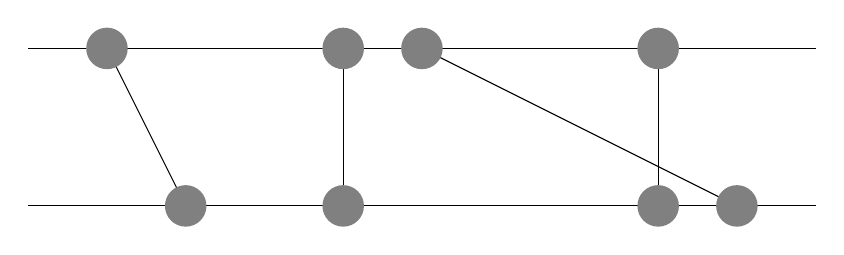
\begin{tikzpicture}
		\draw (0,0) -- (10,0);
		\draw (0,2) -- (10,2);
		% connection
		\draw (1,2) -- (2,0);
		\draw (4,2) -- (4,0);

		\draw (5,2) -- (9,0);
		\draw (8,2) -- (8,0);
		% top
		\node[vertex] at (1,2) {};
		\node[vertex] at (4,2) {};
		\node[vertex] at (5,2) {};
		\node[vertex] at (8,2) {};
		% bottom
		\node[vertex] at (2,0) {};
		\node[vertex] at (4,0) {};
		\node[vertex] at (8,0) {};
		\node[vertex] at (9,0) {};
	\end{tikzpicture}
	\end{center}
\end{frame}


\begin{frame}{Bridges of Kolsberg}
	\bi
		\item Do 2-dimensional DP
		\item<2-> $bridge(i,j)$ - maximum value possible if all bridges start left of $i$ on the north bank, and end left of $j$ on the south bank.
	\ei
	
	\visible<3->{\begin{center} 
	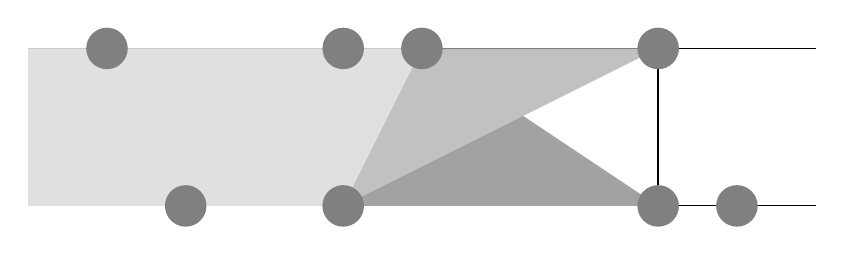
\begin{tikzpicture}
		\draw (0,0) -- (10,0);
		\draw (0,2) -- (10,2);
		% connection
		\draw<3-4,7>[thick] (8,2) -- (8,0);
		\fill<6,7>[gray!60] (0,0) -- (0,2) -- (5,2) -- (8,0) -- cycle;
		\fill<5,7>[gray!40] (0,0) -- (0,2) -- (8,2) -- (4,0) -- cycle;
		\fill<4,7>[gray!20] (0,0) -- (0,2) -- (5,2) -- (4,0) -- cycle;
		
		% top
		\node[vertex] at (1,2) {};
		\node[vertex] at (4,2) {};
		\node[vertex] at (5,2) {};
		\node[vertex] at (8,2) {};
		% bottom
		\node[vertex] at (2,0) {};
		\node[vertex] at (4,0) {};
		\node[vertex] at (8,0) {};
		\node[vertex] at (9,0) {};
	\end{tikzpicture}
	\end{center}}
	
	\visible<7->{\begin{align*}
		bridge(0,j) = &bridge(i,0) = 0\\
		brdige(i,j) = &\mathrm{min} \{bridge(i,j-1), bridge(i-1,j),\\
						&\hspace{1cm} v_i*v_j + bridge(i-1,j-1) \text{ if } t_i = t_j\}\\
	\end{align*}}
\end{frame}


% TODO: Longest increasing subsequence
\begin{frame}{Longest increasing subsequence}
    \bi
\item Given an array $a[0]$, $a[1]$, \ldots, $a[n-1]$ of integers, what is the length of the longest increasing subsequence?
    \vspace{15pt}
\item First, what is a subsequence?
\item If we delete zero or more elements from $a$, then we have a subsequence of $a$
    \vspace{5pt}
\item Example: $a = [5,1,8,1,9,2]$
    \vspace{5pt}
\item $[5,8,9]$ is a subsequence
\item $[1,1]$ is a subsequence
\item $[5,1,8,1,9,2]$ is a subsequence
\item $[]$ is a subsequence
\item $[8,5]$ is \textbf{not} a subsequence
\item $[10]$ is \textbf{not} a subsequence
    \ei
\end{frame}

\begin{frame}{Longest increasing subsequence}
    \bi
\item Given an array $a[0]$, $a[1]$, \ldots, $a[n-1]$ of integers, what is the length of the longest increasing subsequence?
    \vspace{5pt}
\item An increasing subsequence of $a$ is a subsequence of $a$ such that the elements are in (strictly) increasing order
    \vspace{5pt}
\item $[5,8,9]$ and $[1,8,9]$ are the longest increasing subsequences of $a = [5,1,8,1,9,2]$

    \vspace{5pt}
\item How do we compute the length of the longest increasing subsequence?
\item There are $2^n$ subsequences, so we can go through all of them
\item That would result in an $O(n2^n)$ algorithm, which can only handle $n\leq 23$
    \vspace{5pt}
\item What about dynamic programming?

    \ei
\end{frame}

\begin{frame}{Longest increasing subsequence}
    \vspace{20pt}
    \bi
\item Let $\mathrm{lis}(i)$ denote the length of the longest increasing subsequence of the array $a[0]$, $\ldots$, $a[i]$
    \vspace{5pt}
\item Base case: $\mathrm{lis}(0) = 1$
\item What about $\mathrm{lis}(i)$?
    \vspace{10pt}
\item We have the same issue as in the maximum sum problem, so let's try changing perspective
    \ei
\end{frame}

\begin{frame}{Longest increasing subsequence}
    \vspace{40pt}
    \bi
\item Let $\mathrm{lis}(i)$ denote the length of the longest increasing subsequence of the array $a[0]$, $\ldots$, $a[i]$, \textit{that ends at $i$}
    \vspace{5pt}
\item Base case: we don't need one
\item $\mathrm{lis}(i) = \mathrm{max}(1, \mathrm{max}_{j \textrm{ s.t. } a[j] < a[i]} \{ 1 + \mathrm{lis}(j) \})$
    \ei
\end{frame}

\begin{frame}[fragile]{Longest increasing subsequence}
    \begin{minted}[fontsize=\footnotesize]{cpp}
int a[1000];
int mem[1000];
memset(mem, -1, sizeof(mem));

int lis(int i) {
    if (mem[i] != -1) {
        return mem[i];
    }

    int res = 1;
    for (int j = 0; j < i; j++) {
        if (a[j] < a[i]) {
            res = max(res, 1 + lis(j));
        }
    }

    mem[i] = res;
    return res;
}
    \end{minted}
\end{frame}

\begin{frame}[fragile]{Longest increasing subsequence}
    \vspace{30pt}

    \bi
        \item And then the longest increasing subsequence can be found by checking all endpoints:
    \ei

    \begin{minted}{cpp}
int mx = 0;
for (int i = 0; i < n; i++) {
    mx = max(mx, lis(i));
}

printf("%d\n", mx);
    \end{minted}
\end{frame}

\begin{frame}{Longest increasing subsequence}
    \vspace{30pt}
    \bi
        \item Time complexity? \pause
            \vspace{10pt}
        \item There are $n$ possible inputs
        \item Each input is computed in $O(n)$ time, assuming recursive calls are $O(1)$
        \item Total time complexity is $O(n^2)$
            \vspace{10pt}
        \item This will be fast enough for $n \leq 1\ 000$, much better than the brute force method!
    \ei
\end{frame}

\begin{frame}{Longest increasing subsequence}
    \vspace{20pt}
    \bi
      \item Can we do better? \pause - Yes
      \item<3-> Store 
      \bi
    \item<3-> $m[j]$ - index $k$ of the smallest $a[k]$, s.t. there is a LIS of length $j$ ending at $k$
    \item<4-> $p[i]$ - the predecessor of $a[i]$ in the LIS ending at $a[i]$
      \ei
      \item<5-> $a[m[0]],\dots,a[m[sz(m)]]$ is non-decreasing
      \item<6-> Process the array in order
      \bi
    \item<6-> If $a[i] > a[m[sz(m)]]$ we have a new longest LIS
    \item<6-> Else search of the largest value (index: $j$) smaller than $a[i]$ in $a[m[\cdot]]$. We set replace $m[j] = i$
      \ei
      \item<7-> $m[\cdot]$ isn't actually necessary, but only the sequence of values $a[m[\cdot]]$
	  \item<8-> Runtime? \visible<9->{\dots{} Binary Search!}\visible<10->{$\rightarrow \mathcal O(n \log n)$}
    \ei
\end{frame}


\begin{frame}[fragile]{Longest increasing subsequence}
    \begin{minted}[fontsize=\footnotesize]{cpp}
vi LIS(vi A) {
    int N = A.size();
    vi pre(N,-1),erg;
    map<int,int> m;
    map<int,int>::iterator k,l;
    FOR(i, 0, N) if (m.insert(pii(A[i],i)).second) {
        l = k = m.find(A[i]);
        if (l==m.begin()) pre[i]=-1;
        else pre[i]=(--l)->second;
        if ((++k)!=m.end()) m.erase(k);
    }
    for(int j = (--(k = m.end()))->second;j!=-1;j = pre[j])
        erg.push_back(A[j]);
    reverse (erg.begin(),erg.end());
    return erg;
}
    \end{minted}
\end{frame}


\begin{frame}{DP with probabilities}
	\vspace{40pt}
    \bi
        \item Many stochastic problems are at their core DP problems
        \item They describe some transition system with probabilities ...
        \item<2-> ... and ask what the probability to reach a goal state is
        \item<3-> ... or ask how probable it is to reach a goal if you ``play'' optimally
        \item<4-> ... or ask to compute some expected value (when ``playing'' optimally)
    \ei
\end{frame}

\begin{frame}{DP with probabilities}
	\vspace{10pt}
    \bi
        \item We are given a memory game (with regular rules)
        \item You are playing alone and play perfectly
        \item<2-> How many truns do you need on average to finish
        \vspace{10pt}
        \item<3-> What are the DP dimensions?
        \item<4-> $h = $ How many cards are left
		\item<5-> $k = $ How many cards we know (no pairs among them)
        \vspace{10pt}
		\item Systematic analysis of situations!
    \ei
\end{frame}

\begin{frame}{DP with probabilities}
	\bi
		\item There are $h$ cards on the table and we know $k$.
		\item Always take one of the unknown cards first.
		\vspace{10pt}
		\item 1. Card
		\bi
			\item Partner already seen $P=\frac{k}{h-k}$ \\
					$\rightarrow$ take known second, $dp(h-2,k-1)$
			\item Unknown Partner $P=\frac{h-2k}{h-k}$ \\
					$\rightarrow$ take any second
		\ei
		\item 2. Card
		\bi
			\item Matches 1. Card $P=\frac{1}{h-k-1}$\\
					$\rightarrow$ perfect!, $dp(h-2,k)$
			\item Matches known Card $P=\frac{k}{h-k-1}$\\
					$\rightarrow$ take them immediately in the next round, $dp(h-2,k+1)$
			\item Does not match $P = \frac{h-2k-2}{h-k-1}$\\
					$\rightarrow$ just go on, $dp(h,k+2)$
		\ei
		
	\ei
\end{frame}


% TODO: Bitmasks
\begin{frame}{DP over bitmasks}
    \vspace{40pt}
    \bi
        \item Remember the bitmask representation of subsets?
        \item Each subset of $n$ elements are mapped to an integer in the range $0$, \ldots, $2^{n} - 1$
        \item This makes it easy to do dynamic programming over subsets
    \ei
\end{frame}

% TODO: Traveling salesman problem
\begin{frame}{Traveling salesman problem}
    \vspace{10pt}

    \bi
        \item We have a graph of $n$ vertices, and a cost $c_{i,j}$ between each pair of vertices $i, j$. We want to find a cycle through all vertices in the graph so that the sum of the edge costs in the cycle is minimal.

        \vspace{5pt}
        \item This problem is NP-Hard, so there is no known deterministic polynomial time algorithm that solves it

        \vspace{10pt}
        \item Simple to do in $O(n!)$ by going through all permutations of the vertices, but that's too slow if $n > 11$

        \vspace{10pt}
        \item Can we go higher if we use dynamic programming?
    \ei
\end{frame}

\begin{frame}{Traveling salesman problem}
    \vspace{20pt}
    \bi
\item Without loss of generality, assume we start and end the cycle at vertex $0$ and the set of all vertices is $O$
    \vspace{10pt}

\item Let $\mathrm{tsp}(i, S)$ represent the cheapest way to go through the vertices $O \setminus S$ in the graph and back to vertex $0$, if we're currently at vertex $i$ (i.e. we've already visited the vertices $S$ when starting from $0$)

    \vspace{20pt}
\item Base case: $\mathrm{tsp}(i, \textrm{all vertices}) = c_{i,0}$
\item Otherwise $\mathrm{tsp}(i, S) = \mathrm{min}_{\ j \not\in S\ } \{\ c_{i,j} + \mathrm{tsp}(j, S \cup \{j\})\ \}$
    \ei
\end{frame}

\begin{frame}[fragile]{Traveling salesman problem}
    \begin{minted}[fontsize=\scriptsize]{cpp}
const int N = 20;
int c[N][N];
int mem[N][1<<N];
memset(mem, -1, sizeof(mem));

int tsp(int i, int S) {
    if (S == ((1 << N) - 1))
        return c[i][0];
    if (mem[i][S] != -1)
        return mem[i][S];

    int res = oo;
    for (int j = 0; j < N; j++) {
        if (S & (1 << j))
            continue;

        res = min(res, c[i][j] + tsp(j, S | (1 << j)));
    }

    mem[i][S] = res;
    return res;
}
    \end{minted}
\end{frame}

\begin{frame}[fragile]{Traveling salesman problem}
    \vspace{30pt}
    \bi
\item Then the optimal solution can be found as follows:
    \ei

    \vspace{20pt}
    \begin{minted}{cpp}
printf("%d\n", tsp(0, 1<<0));
    \end{minted}
\end{frame}

\begin{frame}{Traveling salesman problem}
    \vspace{30pt}
    \bi
        \item Time complexity? \pause
        \vspace{10pt}
        \item There are $n \times 2^n$ possible inputs
        \item Each input is computed in $O(n)$ assuming recursive calls are $O(1)$
        \item Total time complexity is $O(n^2 2^n)$
            \vspace{10pt}
        \item Now $n$ can go up to about $20$
    \ei
\end{frame}


\begin{frame}{Traveling salesman with teleport}
	\bi
		\item It is not untypical, that we have to adapt a known DP to accommodate for some change in the setting.
		\item<2-> Consider TSP where you have the option to ``teleport'' from some node to some other, taking $s$ time, but you can use this teleport one once.
		\vspace{10pt}
		\item<3-> Introduce a new DP-Dimension: Whether we have used the teleport or not.
		
		\vspace{20pt}
\item<4-> $\mathrm{tsp}(i, \textrm{all vertices},0) = c_{i,0}$
\item<4-> $\mathrm{tsp}(i, S, 0) = \mathrm{min}_{\ j \not\in S\ } \{\ c_{i,j} + \mathrm{tsp}(j, S \cup \{j\},0)\ \}$
\item<4-> $\mathrm{tsp}(i, \textrm{all vertices},1) = \mathrm{min}\{s, c_{i,0}\}$
\item<4-> $\mathrm{tsp}(i, S, 1) = \mathrm{min}\{ \mathrm{min}_{\ j \not\in S\ } \{\ c_{i,j} + \mathrm{tsp}(j, S \cup \{j\},1)\ \}$\\
\hspace{3.1cm} $\mathrm{min}_{\ j \not\in S\ } \{\ s + \mathrm{tsp}(j, S \cup \{j\},0)\ \} \}$
	\ei
\end{frame}

\begin{frame}[fragile]{Traveling salesman problem}
    % http://xkcd.com/399/
    \vspace{40pt}
    \begin{center}
    \ig[scale=0.4]{travelling_salesman_problem.png}
    \end{center}
\end{frame}

\begin{frame}{Recap}
    \vspace{10pt}
    Which types of DP-indices are common in programming contests?
    \bi
		\item $(i)$ -- index on an array (1D Max Sum, LIS, 01-Knapsack, TSP)
		\item $(i,j)$ -- indices on two arrays (Edit distance, LCS)
		\item $(i,j)$ -- subarray of array (optimal matrix multiplication)
		\item $(i,j)$ -- processed values and last selected (bitonic TSP)
		\item $(i)$ -- vertex of a DAG (longest path)
		\item $(s)$ -- state in a transition system (probabilistics)
		\item $(s)$ -- target value (01-knapsack, subsetsum, coin change)
		\item $(s)$ -- subset of a small set (TSP)
    \ei
\end{frame}
		%\item $(i,j)$ -- two indices on the same array (Bitonic TSP)


\end{document}

